\section{Background Theory}
The idea for managing the power consumption was inspired by multiple things.  Mobile phones conserving battery by running basic functions only and hibernation mode on PCs were some of the technologies that led us to want to implement these things.  By gathering all of the power and ground wires to the same point on Tiberius, they could be more easily fed through fuses and connected to relays.  The new fuses were carefully rigged with specially thick wires and specialised sealed rubber holders which could effectively insulate from power surges.

\subsection{Battery Safety}

Some of the obstacles of using Lithium batteries the safety aspects involve as certain Lithium batteries can be volatile, catch fire or even explode.

The LiFe batteries were chosen for this very reason as they were reportedly robust and highly stable, which meant safe to use on Tiberius III.

\subsection{Star Grounding}
In light of optimising circuits and wiring, we tried to adopt star grounding wherever possible.  This meant putting every component's ground into one common ground, known as the star ground point, so that all conductors extend outwards to form a 'star'. This was implemented for all of the high power devices.

\begin{figure}[!htb]
\begin{center}
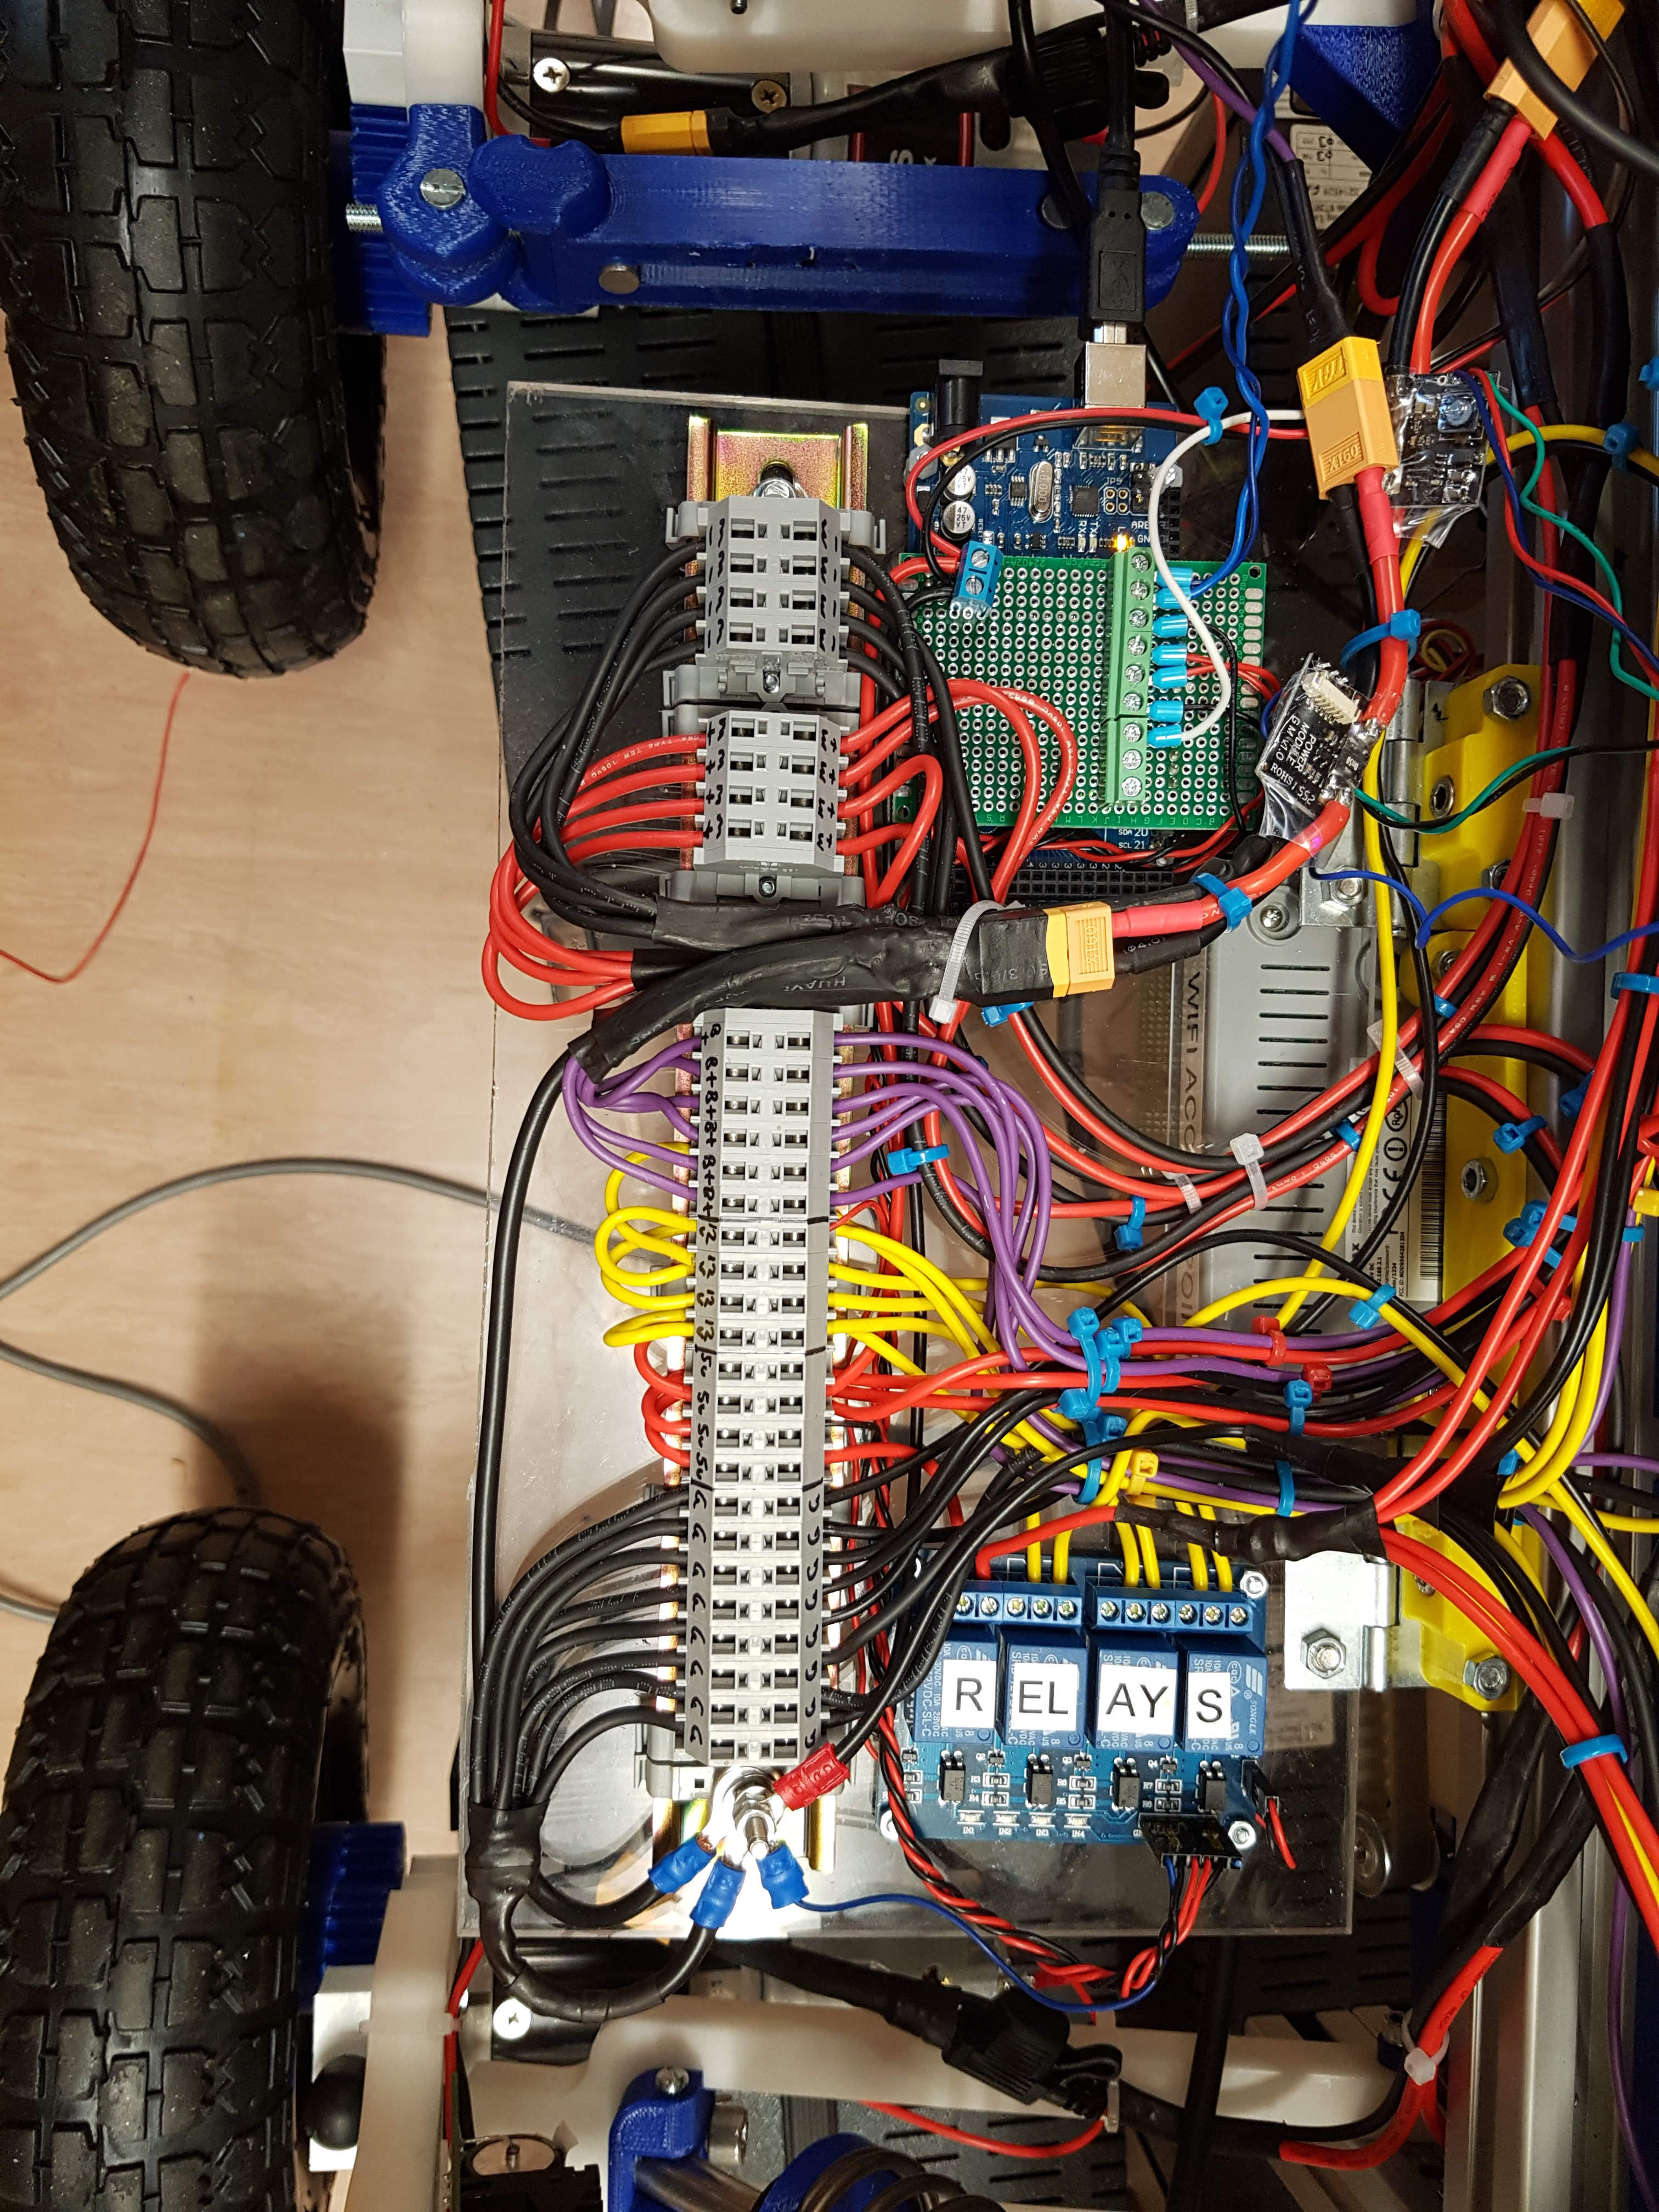
\includegraphics[width=10cm]{cabling.jpg}
\end{center}
\caption{Star Grounding}
\label{fig:Cabling}
\end{figure}